\documentclass[12pt]{article}
\usepackage[utf8]{inputenc}
\usepackage{amsmath}
\usepackage{graphicx}
\usepackage{hyperref}
\usepackage{listings}
\usepackage{float}


\setlength{\parindent}{0pt}
\title{ERTS: Assignment 3}
\author{
Simon Møller, student number: 202204535 \\ 
Mark Myrtoft Bøgelund, student number: 202206634
}
\date{Date: \today}
\lstset{
    language=C++,
    basicstyle=\ttfamily\footnotesize,
    frame=single,
    breaklines=true
}

\begin{document}
\maketitle

\tableofcontents

\newpage

\section{Introduction}
The purpose of this assignment is using design patterns introduced in the
course in a simple embedded system as an example. The specific patterns used
were the State pattern, the Singleton pattern and the Active object pattern.
This report proposes a design for the embedded system using these patterns, and
showcases the implementation and testing of the design.

\section{Design}
The design is divided into three cooperating parts: the system-level state
machine, the substates used while the system is operational, and the active
object responsible for processing change-mode events.

\subsection{System states}

The system-level state pattern models the major states of the embedded system.
\texttt{EmbeddedSystemX} stores a pointer to the current \texttt{SystemState}
and changes state through \texttt{setState}. The concrete states are
\texttt{PowerOnSelfTest}, \texttt{Failure}, \texttt{Initializing}, and
\texttt{Operational}. Each concrete state implements \texttt{invoke} and is
implemented as a Singleton, ensuring that only one instance of each state
exists.

\begin{figure}[H]
    \centering
    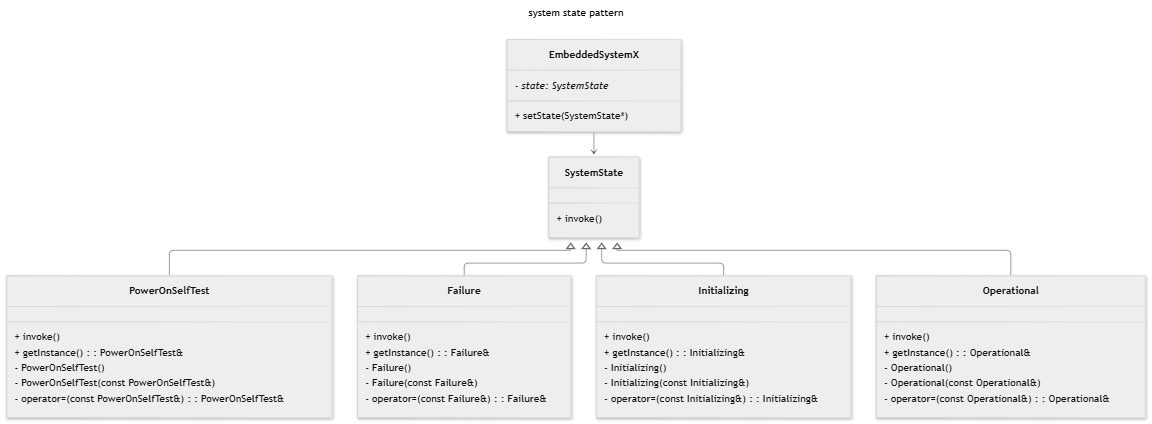
\includegraphics[width=\textwidth]{diagrams/system-state.png}
    \caption{System-level state pattern.}
    \label{fig:system-state}
\end{figure}

\subsection{Operational states}

\texttt{Operational} is itself a state context with a nested state machine.
It stores an \texttt{OperationalState} pointer and controls transitions
between \texttt{Ready}, \texttt{Configuration}, and \texttt{RealTimeLoop}.
This separates the general system lifecycle from the behavior specific to
normal operation. The operational states are also implemented as Singleton.

\begin{figure}[H]
    \centering
    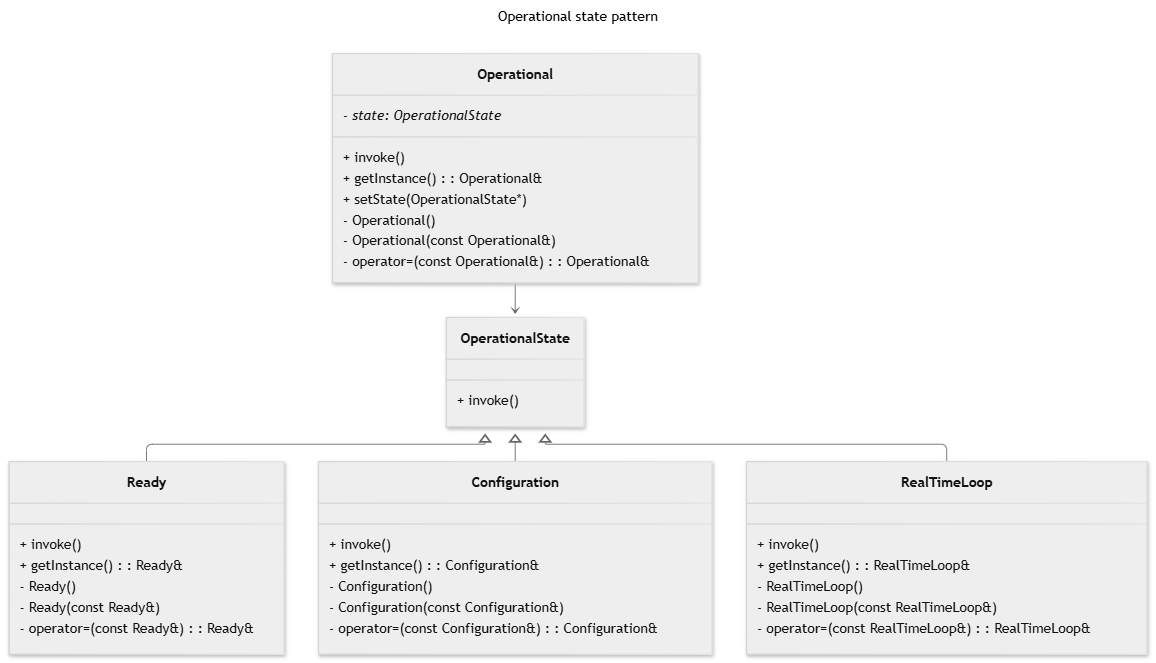
\includegraphics[width=\textwidth]{diagrams/operational-states.png}
    \caption{State pattern for the operational substates.}
    \label{fig:operational-states}
\end{figure}

\subsection{RealTimeLoop with Active Object pattern}

\texttt{RealTimeLoop} acts as the producer side of an active-object design.
When invoked, it creates a \texttt{ChmodeEvent} and pushes it into a
\texttt{ChmodeQueue}. A separate \texttt{ChmodeEventHandler} owns the
processing loop and retrieves events from the queue asynchronously. The event
type identifies the selected change mode, while the queue decouples event
generation from event handling.

\begin{figure}[H]
    \centering
    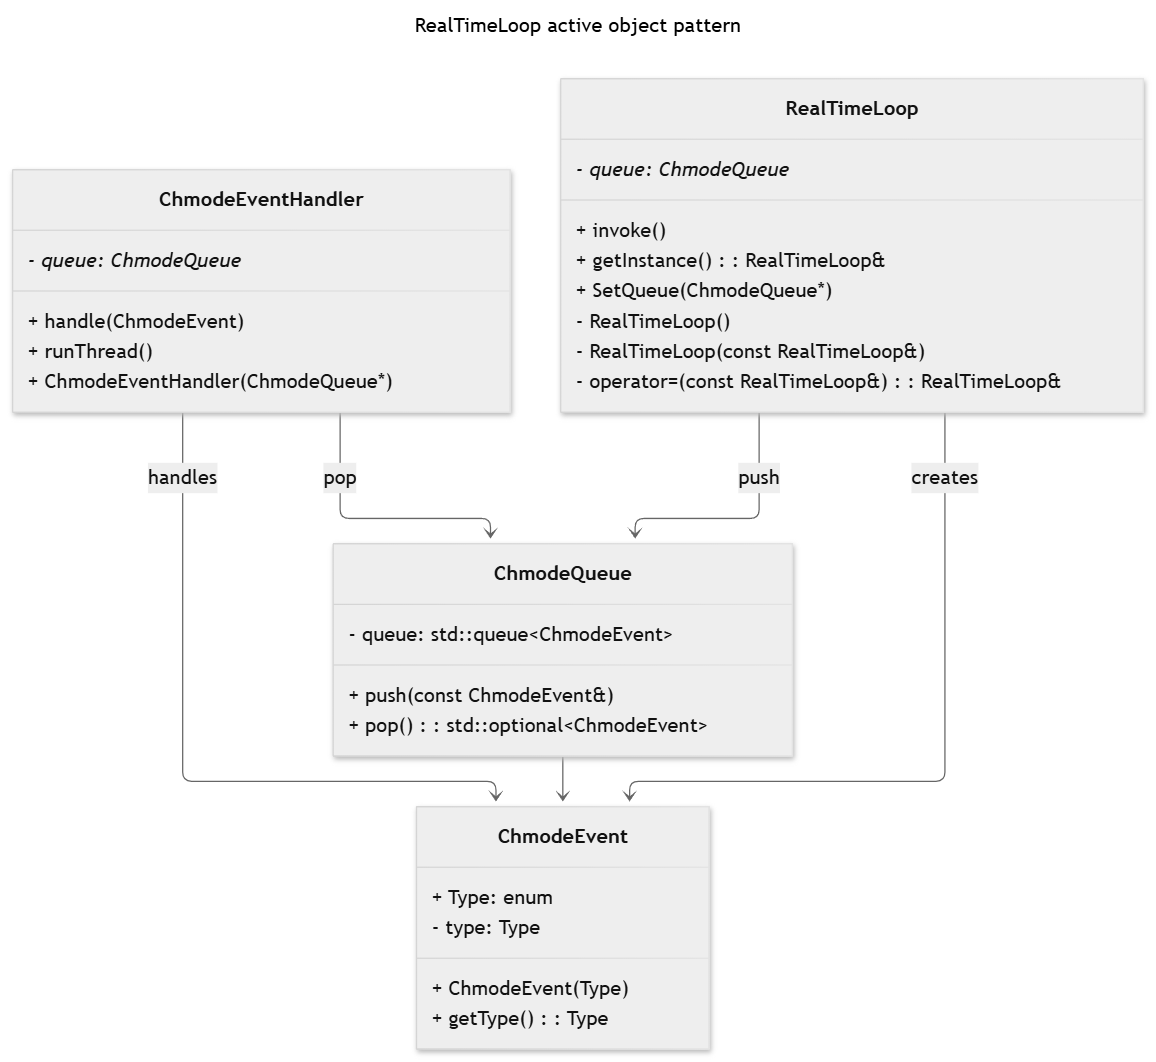
\includegraphics[width=\textwidth]{diagrams/realtime-loop-active-object.png}
    \caption{Active object design for the real-time loop and event handler.}
    \label{fig:realtime-loop}
\end{figure}

\section{Implementation}
The implementation follows the design by separating the state contexts from
their concrete states and by connecting the real-time loop to the event handler
through a queue. The main program creates the contexts and the event handler,
then uses a command loop to request state transitions.

\subsection{Main program loop}

The program creates the queue and handler, connects the queue to the
\texttt{RealTimeLoop}, and starts the handler thread. The user-facing command
loop then delegates transitions to the appropriate context.

\begin{lstlisting}[caption={Main program setup and command loop.}, label={lst:main-setup}, language={C++}]
int main()
{
    EmbeddedSystemX embeddedSystemX;
    ChmodeQueue eventQueue;
    ChmodeEventHandler eventHandler(&eventQueue);
    RealTimeLoop &realTimeLoop = RealTimeLoop::getInstance();
    realTimeLoop.setQueue(&eventQueue);
    Operational &operational = Operational::getInstance();
    std::thread eventHandlerThread(&ChmodeEventHandler::runThread,
                                   &eventHandler);
    embeddedSystemX.setState(&PowerOnSelfTest::getInstance());
    operational.setState(&Ready::getInstance());

    bool running = true;
    while (running)
    {
        std::cout << "\nSelect an action:\n"
                  << "0: Exit\n"
                  << "1: Restart\n"
                  << "2: SelftestFailed\n"
                  << "3: SelftestOk\n"
                  << "4: Initialized\n"
                  << "5: Configure\n"
                  << "6: ConfigurationEnded\n"
                  << "7: Stop\n"
                  << "8: Start/run\n"
                  << "Choice: ";

        int choice = -1;
        if (!(std::cin >> choice))
        {
            std::cin.clear();
            std::cin.ignore(10000, '\n');
            std::cout << "Invalid input\n";
            continue;
        }

        switch (choice)
        {
        case 0:
            running = false;
            break;
        case 1:
            embeddedSystemX.setState(&PowerOnSelfTest::getInstance());
            break;
        case 2:
            embeddedSystemX.setState(&Failure::getInstance());
            break;
        case 3:
            embeddedSystemX.setState(&Initializing::getInstance());
            break;
        case 4:
            embeddedSystemX.setState(&Operational::getInstance());
            break;
        case 5:
            operational.setState(&Configuration::getInstance());
            break;
        case 6:
            operational.setState(&Ready::getInstance());
            break;
        case 7:
            operational.setState(&Ready::getInstance());
            break;
        case 8:
            operational.setState(&realTimeLoop);
            break;
        default:
            std::cout << "Invalid choice\n";
            break;
        }
    }

    eventHandlerThread.join();

    return 0;
}
\end{lstlisting}

\subsection{System state transitions}

\texttt{EmbeddedSystemX::setState} validates the requested transition before
updating the current state. Invalid transitions are rejected, while valid
transitions store the new state and immediately invoke it.

\begin{lstlisting}[caption={Validation and application of a system-state transition.}, label={lst:system-state-transition}, language={C++}]
const bool validTransition =
    (state_ == nullptr && toPowerOnSelfTest) ||
    (fromPowerOnSelfTest && (toFailure || toInitializing)) ||
    (fromFailure && toPowerOnSelfTest) ||
    (fromInitializing && toOperational) ||
    (fromOperational && toPowerOnSelfTest);

if (!validTransition)
{
    std::cerr << "Invalid system state transition\n";
    return;
}

state_ = state;
state_->invoke();
\end{lstlisting}

\subsection{Operational state transitions}

\texttt{Operational} applies the same state-pattern structure at a lower
level. Its validation allows initialization in \texttt{Ready}, transitions
from \texttt{Ready} to either \texttt{Configuration} or
\texttt{RealTimeLoop}, and returns from either of those states to
\texttt{Ready}.

\begin{lstlisting}[caption={Validation and application of an operational-state transition.}, label={lst:operational-state-transition}, language={C++}]
const bool validTransition =
    (state_ == nullptr && toReady) ||
    (fromReady && (toConfiguration || toRealTimeLoop)) ||
    (fromRealTimeLoop && toReady) ||
    (fromConfiguration && toReady);

if (!validTransition)
{
    std::cerr << "Invalid operational state transition\n";
    return;
}

state_ = state;
state_->invoke();
\end{lstlisting}

\subsection{Event creation and queueing}

When \texttt{RealTimeLoop} is invoked, it validates the selected change mode,
converts it to a \texttt{ChmodeEvent}, and pushes the event into the
\texttt{ChmodeQueue}.

\begin{lstlisting}[caption={Creation and queueing of a change-mode event.}, label={lst:event-creation}, language={C++}]
if (queue_ != nullptr)
{
    queue_->push(ChmodeEvent(
        choice == 1 ? ChmodeEvent::Type::Chmode1
                    : ChmodeEvent::Type::Chmode2));
}
\end{lstlisting}

The queue stores events and returns an optional value from \texttt{pop} when an
event is available.

\begin{lstlisting}[caption={Queue insertion and optional event retrieval.}, label={lst:event-queue}, language={C++}]
void push(const ChmodeEvent& event)
{
    queue_.push(event);
}

std::optional<ChmodeEvent> pop()
{
    if (queue_.empty())
        return std::nullopt;

    ChmodeEvent event = queue_.front();
    queue_.pop();
    return event;
}
\end{lstlisting}

\subsection{Event processing}

\texttt{ChmodeEventHandler::runThread} continuously polls the queue. When an
event is available, it passes the event to \texttt{handle}, which dispatches
based on the event type.

\begin{lstlisting}[caption={Polling the queue and dispatching available events.}, label={lst:event-processing}, language={C++}]
void runThread()
{
    while (1)
    {
        if (queue_ != nullptr)
        {
            std::optional<ChmodeEvent> event = queue_->pop();
            if (event.has_value())
                handle(event.value());
        }
    }
}

void handle(const ChmodeEvent& event)
{
    std::cout << "event: "
              << (event.getType() == ChmodeEvent::Type::Chmode1
                      ? "chmode1"
                      : "chmode2")
              << '\n';
}
\end{lstlisting}

\section{Testing}
The tests cover both state-pattern implementations and the active-object
communication through the event queue. Three interactive test cases were
performed: a valid system-state transition, an invalid system-state transition,
and event generation and handling in the real-time loop.

\subsection{Valid state transition}

The program starts in \texttt{PowerOnSelfTest}. Selecting
\texttt{SelftestFailed} requests the transition to \texttt{Failure}. This is a
valid transition according to the system-state rules, so the state is updated
and its \texttt{invoke} method prints \texttt{\{systemstate, Failure\}}.

\begin{figure}[H]
    \centering
    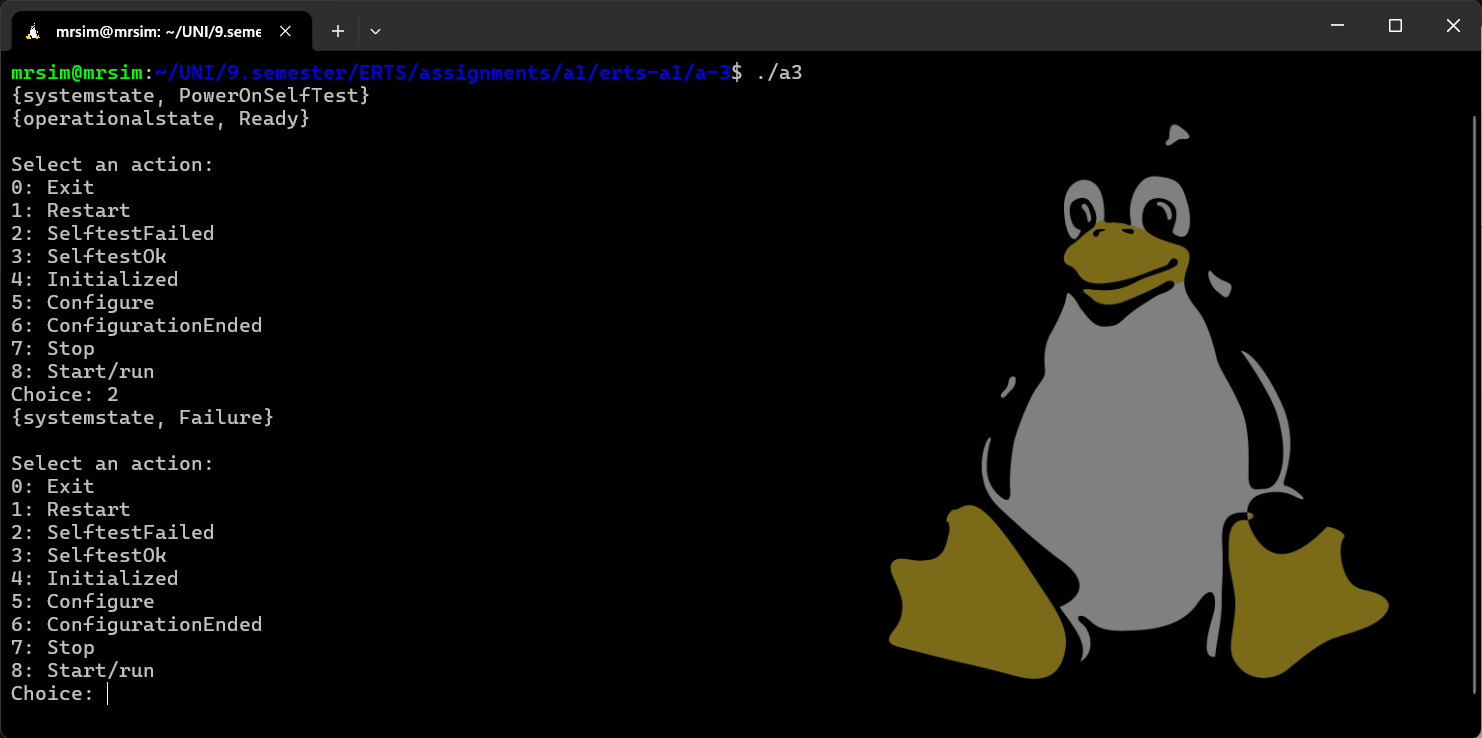
\includegraphics[width=\textwidth]{screenshots/succesfull_state_change.png}
    \caption{Successful transition from \texttt{PowerOnSelfTest} to
        \texttt{Failure}.}
    \label{fig:successful-state-change}
\end{figure}

\subsection{Invalid state transition}

After entering \texttt{Failure}, selecting \texttt{SelftestOk} attempts to
transition directly to \texttt{Initializing}. This transition is not allowed
from \texttt{Failure}; the implementation therefore keeps the current state and
reports \texttt{Invalid system state transition}.

\begin{figure}[H]
    \centering
    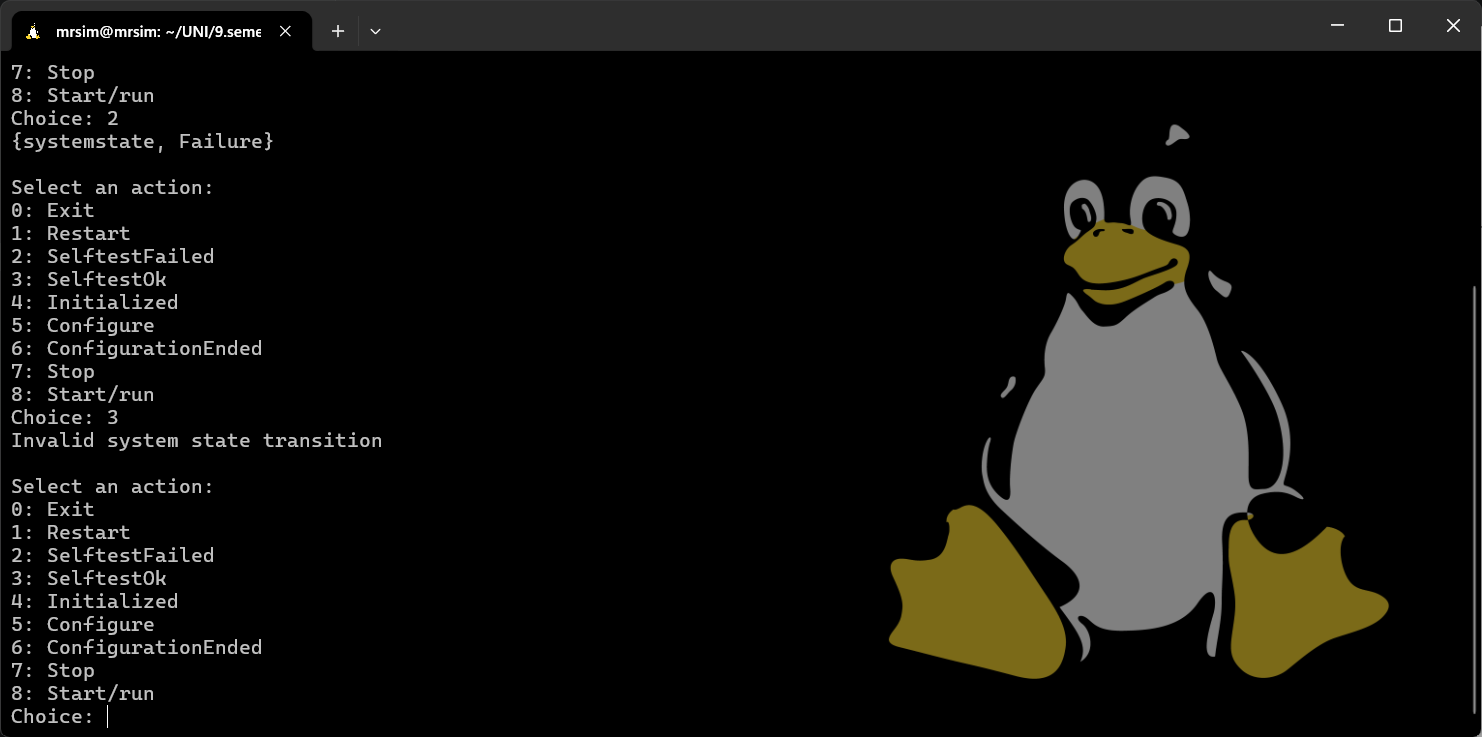
\includegraphics[width=\textwidth]{screenshots/unsuccesfull_state_change.png}
    \caption{Rejected invalid transition from \texttt{Failure} to
        \texttt{Initializing}.}
    \label{fig:unsuccessful-state-change}
\end{figure}

\subsection{Active-object event handling}

To test the active-object pattern, the system is first moved to
\texttt{Operational} and then started with the \texttt{RealTimeLoop} state.
Selecting change mode 1 creates a \texttt{Chmode1} event and pushes it into the
queue. The event handler thread removes the event and prints \texttt{event:
    chmode1}, demonstrating that the event was transferred from the producer to the
handler. Be aware that we haven't handled concurrency for writing to the
console, so the output in the console is not in order, but the event output is
rendered after the prompt for the next input, so it is clear that the event was
handled after the event was created.

\begin{figure}[H]
    \centering
    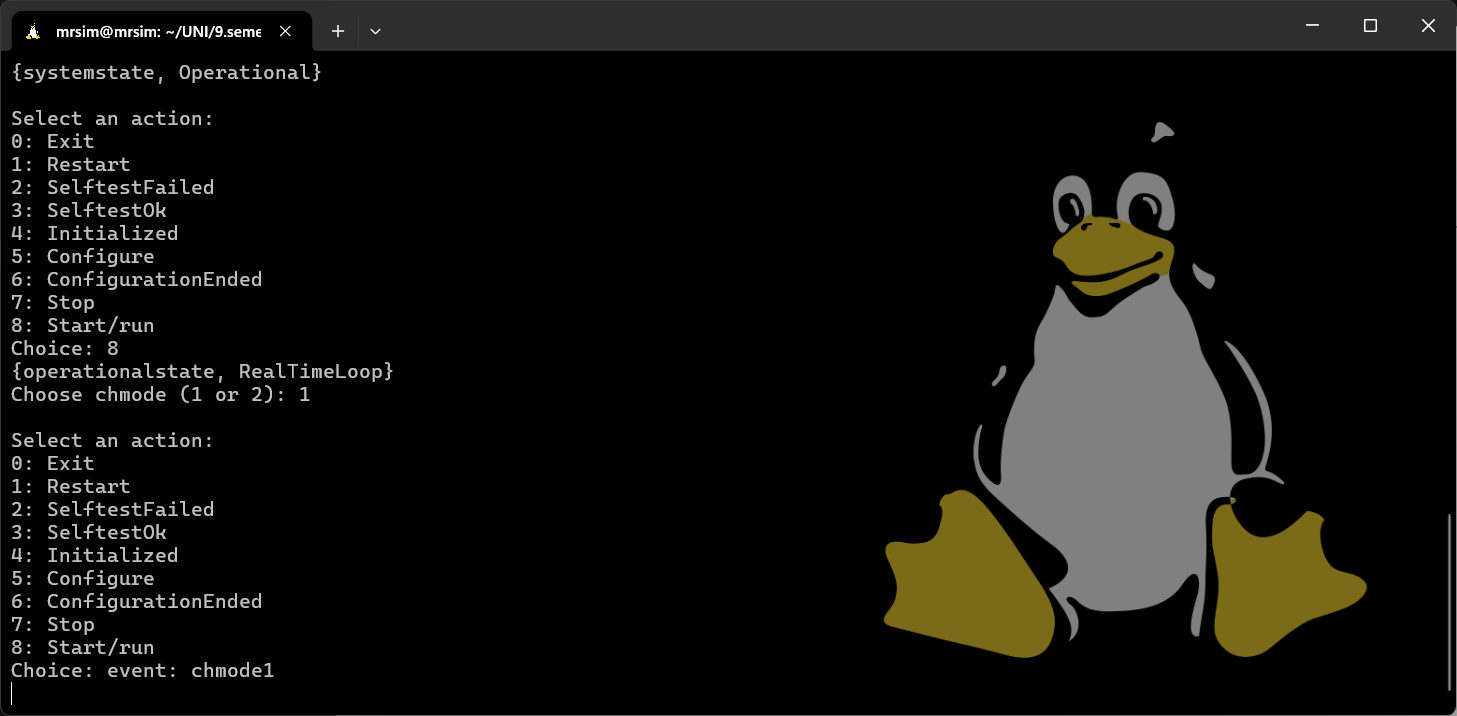
\includegraphics[width=\textwidth]{screenshots/active_object_event.png}
    \caption{A change-mode event being queued and processed by the event
        handler.}
    \label{fig:active-object-event}
\end{figure}

\section{Discussion}
The design and implementation of the embedded system using the state pattern
and active object pattern was successful. The state pattern allowed for clear
separation of concerns between the different states of the system, while the
active object pattern enabled asynchronous event handling. The tests
demonstrated that valid state transitions were handled correctly, invalid
transitions were rejected, and events were successfully passed from the
real-time loop to the event handler.

It should be noted that the utilization of the singleton pattern for the states
may not be suitable for all applications, as it makes the internal state of the
different states persistent across the lifetime of the program. In a more
complex system, it may be necessary to allow for multiple instances of certain
states or to reset their internal state between transitions.

\end{document}